\documentclass{article}
\usepackage{tikz}
\usetikzlibrary{arrows.meta}

\begin{document}

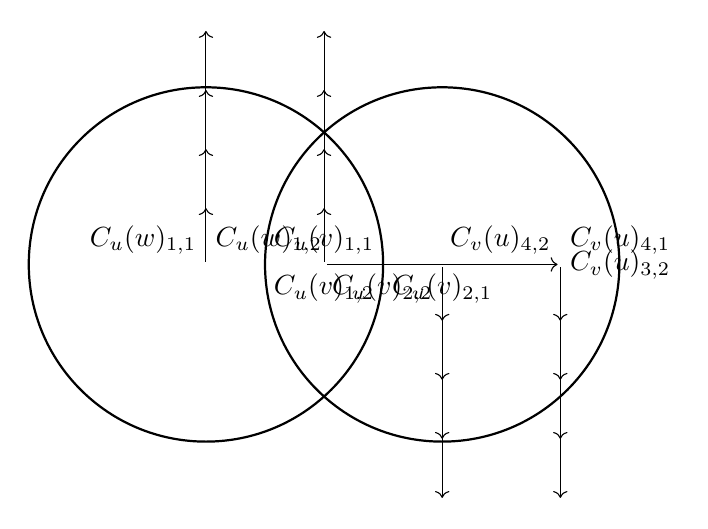
\begin{tikzpicture}[scale=1.5]
    % Define coordinates for the vertices
    \coordinate (A) at (-1,0);
    \coordinate (B) at (0,0);
    \coordinate (C) at (1,0);
    \coordinate (D) at (2,0);
    
    % Draw the cycles
    \draw[thick] (A) circle (1.5cm);
    \draw[thick] (C) circle (1.5cm);
    
    % Label the cycles
    \node at (A) [above left] {$C_u(w)_{1,1}$};
    \node at (A) [above right] {$C_u(w)_{1,2}$};
    \node at (B) [above] {$C_u(v)_{1,1}$};
    \node at (B) [below] {$C_u(v)_{1,2}$};
    \node at (C) [below] {$C_u(v)_{2,1}$};
    \node at (C) [below left] {$C_u(v)_{2,2}$};
    \node at (D) [right] {$C_v(u)_{3,2}$};
    \node at (D) [above right] {$C_v(u)_{4,1}$};
    \node at (D) [above left] {$C_v(u)_{4,2}$};
    
    % Draw the forbidden pairs
    \foreach \x in {1,...,4} {
        \draw[->,shorten >=1pt,shorten <=1pt] (A) -- ++(0,\x*0.5);
        \draw[->,shorten >=1pt,shorten <=1pt] (B) -- ++(0,\x*0.5);
        \draw[->,shorten >=1pt,shorten <=1pt] (C) -- ++(0,-\x*0.5);
        \draw[->,shorten >=1pt,shorten <=1pt] (D) -- ++(0,-\x*0.5);
    }
    
    % Draw the edge uv
    \draw[->,shorten >=1pt,shorten <=1pt] (B) -- (D);
\end{tikzpicture}

\end{document}